\documentclass[lipt]{Article}
\begin{document}
\booktitle{Fanny Shafira Damayanti 1174069 TI2C}

\section{Sejarah Python}

Perintah navigasi direktoriPython adalah Bahasa pemrograman iterperatif multiguna yang berfokus pada tingkat keterbacaan kode. Python merupakan sebuah Bahasa pemrograman yang memiliki  sintaksis kode yang sangat jelas. Python dapat digunakan untuk keperluan pengembangan perangkat lunak dan dapat berjalan di berbagai platform system operasi.

Python dikembangkan oleh Guido van Rossum pada tahun 1990 di CWI, Amsterdam. Nama Python berasal dari sebuah nama acara televisi Monty Python's Flying Circus yang di sukai oleh Guido. 
Semua versi python yang dirilis bersifat open source. Python versi pertama yaitu Python 1.0 yang dirilis pada Januari  1994 dan Python versi terbaru saat ini adalah versi 3.7 yang dirilis pada 27 juni 2018.

\section{Perbedaan Python 2 dan Python 3}

Python 2 di rilis pada tahun 2000, Python 2 dilengkapi dengan berbagai fitur programatikal seperti cycle-detecting garbage collector untuk mengotomasi manajemen memori, peningkatan dukungan untuk Unicode, list comprehension untuk membuat sebuah list berdasarkan list yang sudah ada. Unifikasi pada tipe data Python dan class ke satu hirarki terjadi pada rilis Python 2.2

Python 3 dirilis tahun 2008, Python 3 dilengkapi untuk melakukan perapian pada codebase dan menghapuskan duplikasi (redundancy). Perubahan terbesar pada Python 3 termasuk memasukkan statemen print ke dalam built-in function. Di python 3 tidak memilili backwards compatibility yang ada di Python 2, itu menyebabkan Python 3 mengalami hambatan pada pengadopsiannya. Juga banyak library yang tidak di salin ke Phyton 3, namun pihak pengembang menjelaskan akan menghentikan  dukungan pada Python 2 dan akan menyalin library-library yang ada pada Python 2 ke Python 3. Itu membuat pengguna Python beralih versi dari 2 ke 3.

Perbedaan pada sintaks nya yaitu, di python 2 print diperlakukan seperti statemen ketimbang sebuah function. Contoh
Print “Nama saya Fanny”
Sedangkan di python 3 print diperlakukan sebagai function. Contoh :
Print (“Nama saya Fanny”)

\section{Implementasi dan penggunaan Python di Perusahaan Dunia}
\begin{enumerate}


\item Google adalah perusahaan besar yang menggunakan banyak kode Python di dalam mesin pencarinya. Dan mesin pencari google adalah yang paling terkenal di dunia.

\item Youtube, situs video terbesar dan terpopuler di dunia, sebagian besar kodenya ditulis dalam bahasa Python.

\item Facebook, media sosial terbesar di dunia, menggunakan Tornado, sebuah framework Python untuk menampilkan timeline.

\item Instagram, siapa yang tidak kenal. Instagram menggunakan Django, framework python sebagai mesin pengolah sisi server dari aplikasinya.

\item Pinterest, banyak menggunakan python untuk membangun aplikasinya.

\item Dropbox, barangkali Anda adalah salah seorang pengguna layanan ini. Dropbox menggunakan python baik di sisi server maupun di sisi pengguna layanannya.

\item Quora, salah satu situs tanya jawab terbesar di dunia, dibangun menggunakan Python.

\item NASA, badan antariksa Amerika ini menggunakan Python untuk bidang sainsnya.

\item NSA, badan mata – mata Amerika banyak menggunakan Python untuk analisa kriptografi dan intelijen.

\item Industrial Light and Magic, Pixar, banyak menggunakan Python dalam animasi movie.

\item Blender, Maya, software pembuat animasi 3D terkenal, menggunakan Python sebagai salah satu bahasa skrip pemrogramannya.

\item Raspberry Pi, komputer mini yang banyak digunakan sebagai mikrokontroller, menggunakan Python sebagai bahasa utamanya.

\item ESRI, produsen terkenal pembuat software pemetaan GIS banyak menggunakan Python di produknya.


\end{enumerate}

\section{Instalasi}
\subsection{Python}
\begin{enumerate}
\item Buka File python

\item Pilih Pengguna

Pilih ‘Install for all users’ agar bisa dipakai untuk semua user di komputernya.

\begin{figure}[htbp]
\centerline{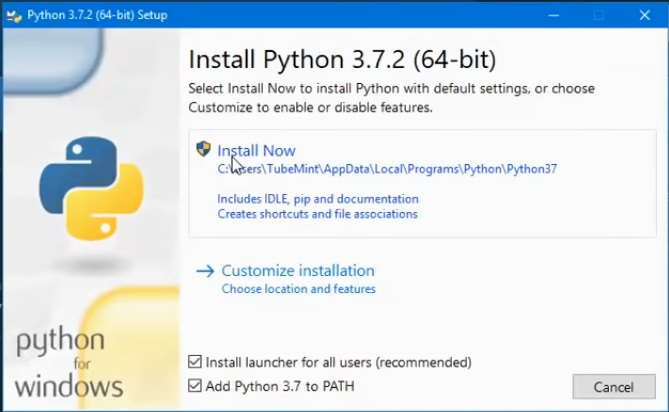
\includegraphics{chapters/gambar/start.jpg}}
\caption{Pilih pengguna.}
\label{fig}
\end{figure}

\item Lokasi Instalasi

Tentukan lokasi python akan diinstal. 

\item Kostumisasi

Pada tahapan ini, kita akan menentukan fitur-fitur yang akan diinstal.

\item selesai
\begin{figure}[htbp]
\centerline{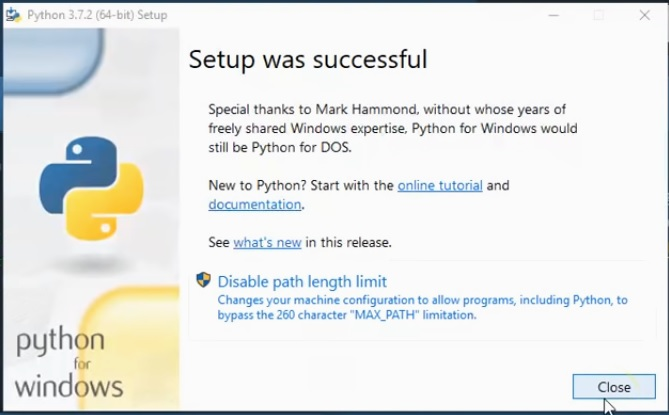
\includegraphics{chapters/gambar/finish.jpg}}
\caption{selesai.}
\label{fig}
\end{figure}
\end{enumerate}

\subsection{Anaconda}
\begin{enumerate}
\item Download installer anaconda terlebih dahulu 

\item Kemudian pilih lokasi yang diinginkan.
\begin{figure}[htbp]
\centerline{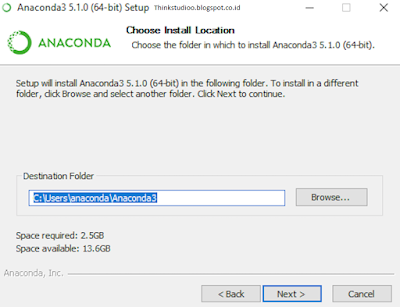
\includegraphics{1.png}}
\caption{Pilih lokasi.}
\label{fig}
\end{figure}

\item Kemudian dipilih add anaconda to PATH atau tidak kemudian klik next.
\begin{figure}[htbp]
\centerline{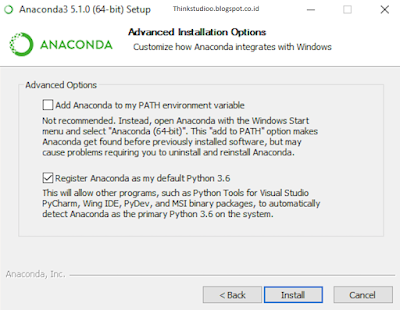
\includegraphics{chapters/gambar/2.png}}
\caption{add anaconda to path.}
\label{fig}
\end{figure}

\item Klik tombol Install. 

\item Untuk menginstal VS Code, klik tombol Install Microsoft VS Code. Setelah instalasi selesai, klik tombol Next Atau untuk menginstal Anaconda tanpa VS code, klik tombol skip. 
\begin{figure}[htbp]
\centerline{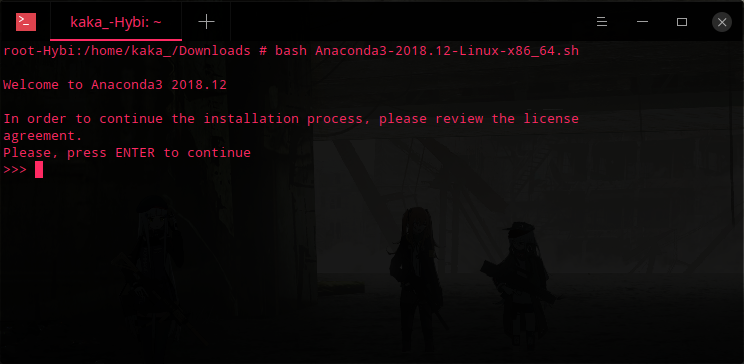
\includegraphics{chapters/gambar/3.png}}
\caption{Install vs code.}
\label{fig}
\end{figure}

\item Setelah instalasi yang sukses, Kalian akan melihat kotak dialog "Thanks for installing Anaconda3"
\begin{figure}[htbp]
\centerline{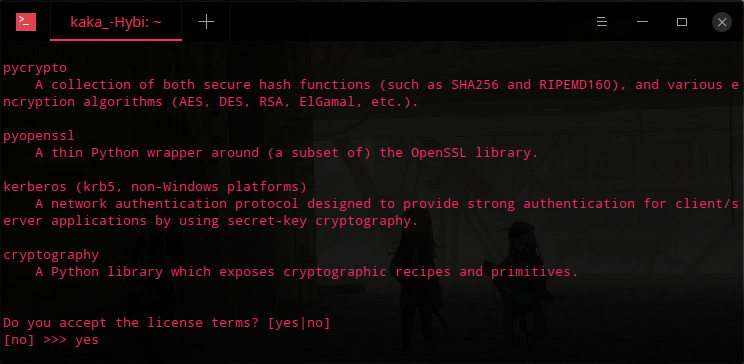
\includegraphics{chapters/gambar/4.png}}
\caption{Selesai.}
\label{fig}
\end{figure}

\end{enumerate}

\section{Cara Pemakaian Script dan Intepreter Python}
\subsection{Cara pemakaian script  python}

Pada Python, file hanya dikelompokkan menjadi dua tipe:

\begin{enumerate}


\item File Teks: File yang berisi teks. Setiap baris teks memiliki EOL (End of Line).

Contoh: TXT, MD, CSV, JSON, dsb.

\item File Binary: File yang bukan teks, hanya bisa diproses oleh program tertentu yang memahami strukturnya.

Contoh: EXE, JPG, MKV, M4A, 3GP, dsb.
\end{enumerate}

Python sudah menyediakan fungsi open() untuk membaca dan menulis file.

Fungsi ini memiliki dua parameter, yaitu nama file dan mode.

Objek file adalah variabel objek yang menampung isi file. Kita bisa melakukan pemrosesan file berkatnya.

Nama file bisa kita isi langsung apabila file-nya terletak dalam satu direktori dengan skrip python. Namun, apabila terletak di direktori yang berbeda, maka kita harus memberikan alamat path file-nya.

Ada beberapa mode yang tersedia:
\begin{enumerate}

\item “r”	 = hanya baca saja
\item “w”	= akses untuk menulis file, jika file sudah ada, maka file akan di replace dan diganti dengan yang baru ditulis
\item “a”	= digunakan untuke append atau menambah data ke file, artinya jika sudah ada data dalam file, maka akan ditambahkan dan tidak di-replace
\item “r+” =	digunakan untuk membaca sekaligus menulis data ke file
\end{enumerate}

\subsection{Interpreter Python}
\begin{enumerate}
\item CyPython
\item PyPy
\item Jython
\item IronPython
\item PythonNet
\end{enumerate}

\section{Cara Pemakaian Spyder termasuk variable explorer}

Explorer Variabel menunjukkan konten namespace (semua referensi objek global, seperti variabel, fungsi, modul, dll.) dari sesi Konsol IPython yang saat ini dipilih, dan memungkinkan untuk berinteraksi dengan mereka melalui berbagai editor berbasis GUI.

\begin{figure}[htbp]
\centerline{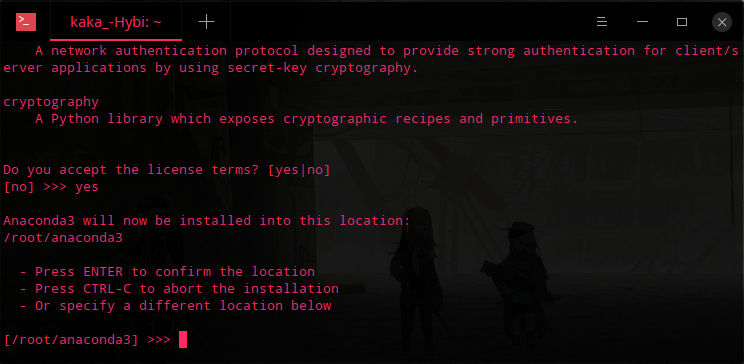
\includegraphics{chapters/gambar/5.png}}
\caption{Variable Explorer.}
\label{fig}
\end{figure}

\section{Mencoba Python}
sintax dasar = print ("Hello Fanny")

\begin{figure}[htbp]
\centerline{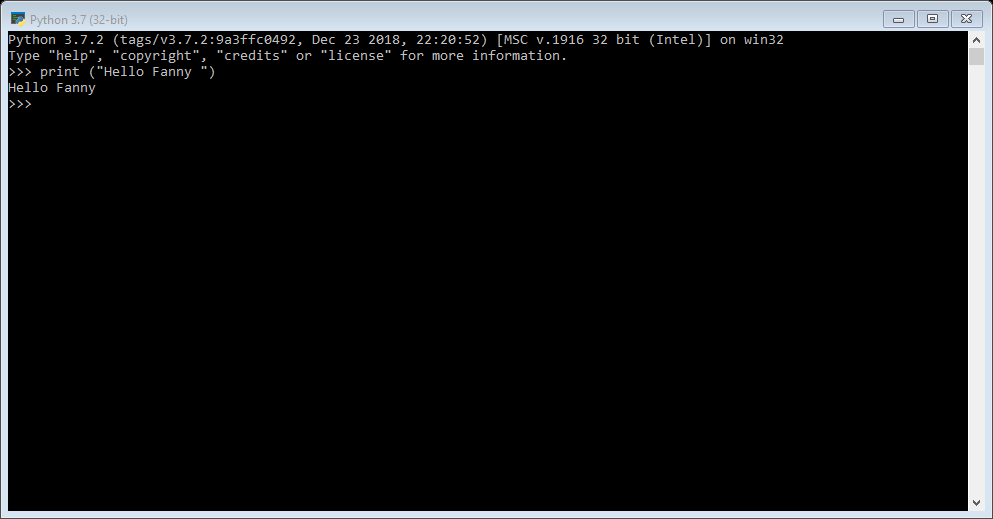
\includegraphics{chapters/gambar/6.png}}
\caption{Sintax dasar python.}
\label{fig}
\end{figure}

\section{Identasi}
Indentasi adalah bagian paragraf yang menjorok ke dalam pada baris-baris paragraph. Pengaturan indentasi atau penggeseran paragraf baik ke kiri maupun ke kanan dapat dilakukan dengan berbagai cara. 

Python memanfaatkan indentasi untuk membuka/menutup fungsi. untuk membuat identasi yang seragam, contoh nya ketika menggunakan notepad++ setting perintah Tab menjadi indentasi 4 karakter spasi , dengan memilih Setting -> Preferences ceklist box Replace by Space dengan Tab Size = 4.


\end{document}